\begin{figure}[h]
	\centering
	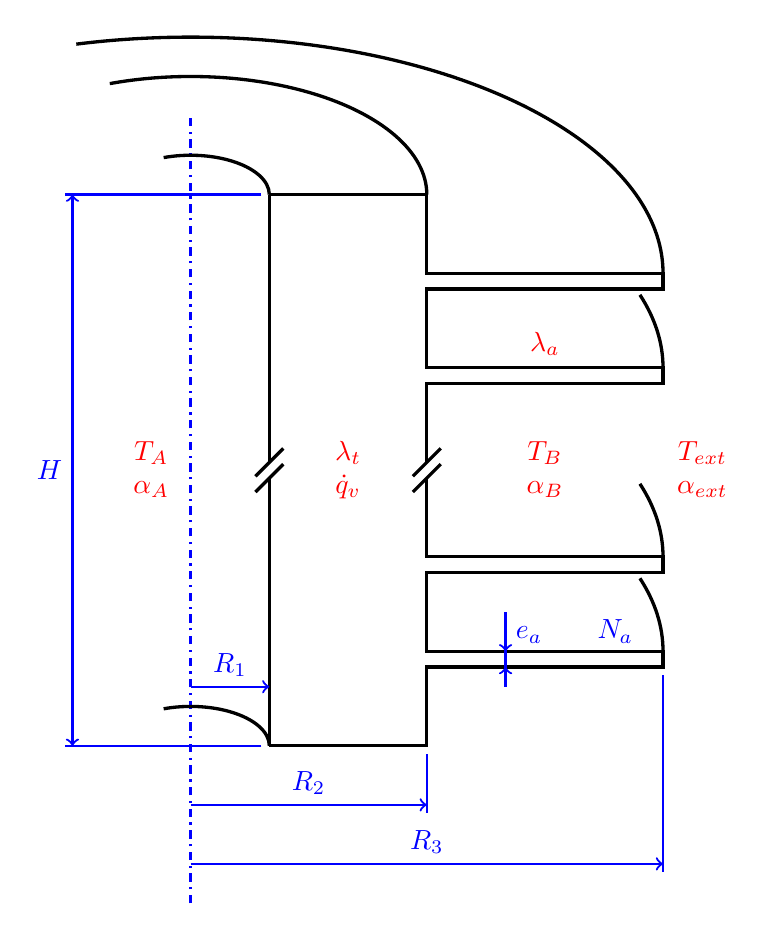
\begin{tikzpicture}
		% Structure
		\draw[black, very thick] (1,0) -- ++(2,0) 
		-- ++(0,1) -- ++(3,0) -- ++(0,0.2) -- ++(-3,0)
		-- ++(0,1) -- ++(3,0) -- ++(0,0.2) -- ++(-3,0)
		-- ++(0,1);
		\draw[black, very thick] (3,3.6) -- ++(0,1) -- ++(3,0) -- ++(0,0.2) -- ++(-3,0)
		-- ++(0,1) -- ++(3,0) -- ++(0,0.2) -- ++(-3,0)
		-- ++(0,1) -- ++(-2,0);
		\draw[black, very thick] (1,0) -- ++(0,3.4);
		\draw[black, very thick] (1,3.6) -- ++(0,3.4);
		\draw[black, very thick] ({3+0.25*cos(225)},{3.4+0.25*sin(225)}) -- ++({0.5*cos(45)},{0.5*sin(45)});
		\draw[black, very thick] ({3+0.25*cos(225)},{3.6+0.25*sin(225)}) -- ++({0.5*cos(45)},{0.5*sin(45)});
		\draw[black, very thick] ({1+0.25*cos(225)},{3.4+0.25*sin(225)}) -- ++({0.5*cos(45)},{0.5*sin(45)});
		\draw[black, very thick] ({1+0.25*cos(225)},{3.6+0.25*sin(225)}) -- ++({0.5*cos(45)},{0.5*sin(45)});
		% Eje
		\draw[blue, thick, dashdotted] (0,-2) -- ++(0,10);
		% Cota H
		\draw[<->, blue, thick] (-1.5,0) -- node[midway, left]{$H$} ++(0,7);
		\draw[blue, thick] (0.9,0) -- ++(-2.5,0);
		\draw[blue, thick] (0.9,7) -- ++(-2.5,0);
		% Cota ea
		\draw[->, blue, thick] (4,0.75) -- ++(0,0.25);
		\draw[<-, blue, thick] (4,1.2) -- node[midway, right]{$e_a \qquad N_a$}++(0,0.5);
		\draw[-, blue, thick] (4,0.75) -- ++(0,0.95);
		% Cota R1
		\draw[->, blue, thick] (0,0.75) -- node[midway, above]{$R_1$}++(1,0);
		% Cota R2
		\draw[->, blue, thick] (0,-0.75) -- node[midway, above]{$R_2$}++(3,0);
		\draw[blue, thick] (3,-0.85) -- ++(0,0.75);
		% Cota R3
		\draw[->, blue, thick] (0,-1.5) -- node[midway, above]{$R_3$}++(6,0);
		\draw[blue, thick] (6,-1.6) -- ++(0,2.5);
		% Texto fluido A
		\node[red] at (-0.5,3.5) {\begin{tabular}{c} $T_A$ \\ $\alpha_A$ \end{tabular}};
		% Texto fluido B
		\node[red] at (4.5,3.5) {\begin{tabular}{c} $T_B$ \\ $\alpha_B$ \end{tabular}};
		% Texto tubo
		\node[red] at (2,3.5) {\begin{tabular}{c} $\lambda_t$ \\ $\dot{q}_v$ \end{tabular}};
		% Texto tubo
		\node[red] at (6.5,3.5) {\begin{tabular}{c} $T_\text{ext}$ \\ $\alpha_\text{ext}$ \end{tabular}};
		% Texto aleta
		\node[red] at (4.5,5.1) {$\lambda_a$};
		% Elipses
		\draw[black, very thick] (1,0) arc(0:110:1cm and 0.5cm);
		\draw[black, very thick] (1,7) arc(0:110:1cm and 0.5cm);
		\draw[black, very thick] (3,7) arc(0:110:3cm and 1.5cm);
		\draw[black, very thick] (6,6) arc(0:104:6cm and 3cm);
		\draw[black, very thick] (6,4.8) arc(0:18:6cm and 3cm);
		\draw[black, very thick] (6,2.4) arc(0:18:6cm and 3cm);
		\draw[black, very thick] (6,1.2) arc(0:18:6cm and 3cm);
	\end{tikzpicture}
	\caption{Geometria i propietats termofísiques del problema.}
	\label{fig:plantejament_problema}
\end{figure}


\clearpage
\subsection{Equacions de discretització}

\subsubsection{Node extrem $i = 0$}

El node $i = 0$ és a la cara interna del cilindre, en contacte amb el fluid $A$. El diagrama de fluxos de calor es mostra a la figura \ref{fig:fluxos_calor_node_0}.

\begin{figure}[h]
	\centering
	\begin{tikzpicture}
		% Structure
		\draw[black, line width=0.5mm] (-0.5,0) -- ++(4,0);
		\draw[black, line width=0.5mm] (-0.5,3) -- ++(4,0);
		\draw[black, line width=0.5mm] (1,0) -- ++(0,3);
		\draw[black, line width=0.25mm, dashed] (3,0) -- ++(0,3);
		% Axis
		\draw[blue, line width=0.25mm, dashdotted] (0,-0.5) -- ++(0,4);
		% Nodes
		\filldraw[nodeColor] (1,1.5) circle (3pt);
		\filldraw[nodeColor] (2,1.5) circle (3pt);
		% Text
		\node[nodeColor] at (0.75,1) {$P$};
		\node[nodeColor] at (2,1) {$E$};
		% Heat flows
		\draw[->, tempColor, line width=0.25mm] (0.2,1.5) -- ++(0.8,0);
		\draw[->, tempColor, line width=0.25mm] (1,1.5) -- ++(0.8,0);
		% Text
		\node[tempColor] at (0.5,1.8) {$\dot{Q}_\text{\tiny{conv}}$};
		\node[tempColor] at (1.4,1.8) {$\dot{Q}_e$};
		\node[tempColor] at (-0.5,1.5) {\begin{tabular}{c} $T_A$ \\ $\alpha_A$ \end{tabular}};
	\end{tikzpicture}
	\captionsetup{width=0.6\textwidth}
	\caption{Fluxos de calor en el node $i = 0$.}
	\label{fig:fluxos_calor_node_0}
\end{figure}

Comencem plantejant el primer principi de la Termodinàmica en règim transitori sobre el node $P$, sabent que $V_P = 0$.
\begin{equation} \label{eq:node_0_ppt}
	\pdv{t} \int_{V_p} \rho u \dd{V} = \sum \dot{Q}_P = 0
\end{equation}
Integrant el terme dret de \ref{eq:node_0_ppt} entre els intants $t^n$ i $t^{n+1}$, obtenim:
\begin{equation} \label{eq:node_0_eq_1}
	\int_{t^{n}}^{t^{n+1}} \sum \dot{Q}_P \dd{t} =
	\left( \beta \sum \dot{Q}_P^{n+1} + (1 - \beta) \sum \dot{Q}_P^n \right) \Delta t = 0
\end{equation}
on el flux de calor net a través de $P$ en un instant qualsevol $t^n$ és
\begin{equation} \label{eq:node_0_fluxe_calor}
	\dot{Q}_P^n = 
	\dot{Q}_\text{conv,A}^n - \dot{Q}_e^n =
	\alpha_A^n \left( T_A^n - T_P^n \right) S_\text{conv,A} + \lambda_e^n \frac{T_E^n - T_P^n}{d_{PE}} S_e
\end{equation}
Introduint \eqref{eq:node_0_fluxe_calor} en \eqref{eq:node_0_eq_1} i desenvolupant, obtenim
\begin{equation}
	\beta \left( \frac{\lambda_e^{n+1} S_e}{d_{PE}} + \alpha_A^{n+1} S_\text{conv,A} \right) T_P^{n+1} = 
	\beta \frac{\lambda_e^{n+1} S_e}{d_{PE}} T_E^{n+1} + 
	\beta \alpha_A^{n+1} T_A^{n+1} S_\text{conv,A} + 
	\left( 1 - \beta \right) \sum \dot{Q}_P^n
\end{equation}
Definim els següents coeficients de discretització pel node d'estudi:
\begin{align}
	a_W[0] &= 0												\\
	a_E[0] &= \beta \frac{\lambda_e^{n+1} S_e}{d_{PE}} 		\\
	a_P[0] &= a_W[0] + a_E[0] + \beta \alpha_A^{n+1} S_\text{conv,A}  	\\
	b_P[0] &= \beta \alpha_A^{n+1} T_A^{n+1} S_\text{conv,A} + (1 - \beta) \sum \dot{Q}_P^n
\end{align}
Les posicions dels nodes són $R[0] = R_A$ i $R[1] = R_A + \frac{\Delta R}{2}$. A partir d'aquestes, tenim
\[
	S_e = S_\text{conv,A} = 2 \pi R_A H \qquad d_{PE} = R[1] - R[0] = \frac{\Delta R}{2}
\]
L'equació de discretització que obtenim pel node $i = 0$ és
\begin{equation}
	a_P[0] \, T^{n+1}[0] = a_W[0] \, T^{n+1}[-1] + a_E[0] \, T^{n+1}[1] + b_P[0]
\end{equation}

\clearpage

\subsubsection{Nodes interns $i = 1 \divisionsymbol N$}

Els nodes interns són aquells amb índexs $1 \leq i \leq N$. El diagrama de fluxos de calor per aquests nodes es mostra a la figura \ref{fig:fluxos_calor_nodes_inters_tub}.

\begin{figure}[ht]
	\centering
	\begin{tikzpicture}
		% Structure
		\draw[black, line width=0.5mm] (-0.5,0) -- (6.5,0);
		\draw[black, line width=0.5mm] (-0.5,3) -- (6.5,3);
		% Control volumes
		\draw[black, line width=0.25mm, dashed] (0,0) -- ++(0,3);
		\draw[black, line width=0.25mm, dashed] (2,0) -- ++(0,3);
		\draw[black, line width=0.25mm, dashed] (4,0) -- ++(0,3);
		\draw[black, line width=0.25mm, dashed] (6,0) -- ++(0,3);
		% Nodes
		\filldraw[nodeColor] (1,1.5) circle (3pt);
		\filldraw[nodeColor] (3,1.5) circle (3pt);
		\filldraw[nodeColor] (5,1.5) circle (3pt);
		% Heat flows
		\draw[->, tempColor, line width=0.25mm] (1.6,1.5) -- ++(0.8,0);
		\draw[->, tempColor, line width=0.25mm] (3.6,1.5) -- ++(0.8,0);
		\draw[->, tempColor, line width=0.25mm] ({3+0.5*cos(225)},{1.5+0.5*sin(225)}) arc (225:-45:0.5);
		% Text
		\node[tempColor] at (1.7,1.8) {$\dot{Q}_e$};
		\node[tempColor] at (4.3,1.8) {$\dot{Q}_w$};
		\node[tempColor] at (3,2.3) {$\dot{Q}_{VP}$};
		\node[nodeColor] at (1,1) {$W$};
		\node[nodeColor] at (3,1) {$P$};
		\node[nodeColor] at (5,1) {$E$};
	\end{tikzpicture}
	\captionsetup{width=0.6\textwidth}
	\caption{Fluxos de calor en els nodes interns del tub $\left( i = 1 \divisionsymbol N \right)$.}
	\label{fig:fluxos_calor_nodes_inters_tub}
\end{figure}

Per trobar l'equació de discretització, comencem plantejant el primer principi de la Termodinàmica en règim transitori sobre el volum de control del node $P$:
\begin{equation} \label{eq:nodes_interns_ppt}
	\pdv{t} \int_{V_P} \rho u \dd{V} = \sum \dot{Q}_P
\end{equation}
No coneixem l'expressió de l'energia interna en el VC $P$. Per aquest motiu definim l'energia interna mitja del volum de control com
\begin{equation}
	\overline{u}_P = \frac{1}{\rho_P V_P} \int_{V_P} \rho u \dd{V}
\end{equation}
Atès que $\rho_P$ i $V_P$ són constants, podem escriure \eqref{eq:nodes_interns_ppt} com:
\begin{equation} 
	\pdv{\left(\rho_P V_P \overline{u}_P\right)}{t} = 
	\rho_P V_P \pdv{\overline{u}_P}{t} =
	\sum \dot{Q}_P
\end{equation}
Integrant entre dos temps $t^n$ i $t^{n+1}$ tenim
\begin{equation} \label{eq:nodes_interns_eq_2}
	\int_{t^n}^{t^{n+1}} \rho_P V_P \pdv{\overline{u}_P}{t} \dd{t} = 
	\int_{t^n}^{t^{n+1}} \sum \dot{Q}_P \dd{t}
\end{equation}
Desenvolupem primerament el terme esquerre de \eqref{eq:nodes_interns_eq_2}. Sabem que l'energia interna és una funció de punt, per tant la integral de $\partial \overline{u}_P / \partial t$ entre els instants $t^n$ i $t^{n+1}$ no depèn del procès seguit sino dels estats inicial i final. Podem aproximar el sòlid per un sòlid semiperfecte i fer $\overline{u}_P \approx u_P$. Així mateix, sabem que $\dd{u} = c_p \dd{T}$. Amb aquestes deduccions, el terme esquerre de \eqref{eq:nodes_interns_eq_2} queda
\begin{align}
	\int_{t^n}^{t^{n+1}} \rho_P V_P \pdv{\overline{u}_P}{t} \dd{t} 			&= 
	\rho_P V_P  \int_{t^n}^{t^{n+1}} \pdv{\overline{u}_P}{t} \dd{t} = 
	\rho_P V_P \left( \overline{u}_P^{n+1} - \overline{u}_P^n \right) \nonumber  \\ 	&\approx 
	\rho_P V_P \left( u_P^{n+1} - u_P^n \right) = 
	\rho_P V_P \overline{c}_{p_P} \left( T_P^{n+1} - T_P^n \right) \label{eq:nodes_interns_terme_esquerre}
\end{align}
on $\overline{c}_{p_P}$ és
\[
	\overline{c}_{p_P} = \frac{1}{T_P^{n+1} - T_P^n} \int_{T_P^n}^{T_P^{n+1}} c_p(\tau) \dd{\tau} \approx c_p
\]
El terme dret de \eqref{eq:nodes_interns_eq_2} desenvolupat queda
\begin{equation} \label{eq:nodes_interns_terme_dret}
	\int_{t^n}^{t^{n+1}} \sum \dot{Q}_P \dd{t} = 
	\left( \beta \sum \dot{Q}_P^{n+1} + (1 - \beta) \sum \dot{Q}_P^n \right) \Delta t
\end{equation}
Introduint \eqref{eq:nodes_interns_terme_esquerre} i \eqref{eq:nodes_interns_terme_dret} en \eqref{eq:nodes_interns_eq_2} obtenim
\begin{equation} \label{eq:nodes_interns_eq_3}
	\rho_P V_P \overline{c}_{p_P} \frac{T_P^{n+1} - T_P^n}{\Delta t} = 
	\beta \sum \dot{Q}_P^{n+1} + (1 - \beta) \sum \dot{Q}_P^n	
\end{equation}
on el flux de calor net en un instant general $t^{n}$ és
\begin{equation} \label{eq:nodes_interns_fluxe_calor}
	\sum \dot{Q}_P^n = \dot{Q}_w^n - \dot{Q}_e^n + \dot{Q}_{VP}^n \approx
	-\lambda_w^n \frac{T_P^n - T_W^n}{d_{PW}} S_w + 
	\lambda_e^n \frac{T_E^n - T_P^n}{d_{PE}} S_e + 
	\dot{q}_V^n V_P
\end{equation}
Desenvolupant \eqref{eq:nodes_interns_eq_3} arribem a
\begin{multline}
	\left[ 
	\beta \left( \frac{\lambda_w^{n+1} S_w}{d_{PW}} + \frac{\lambda_e^{n+1} S_e}{d_{PE}} \right) + 
	\frac{\rho_P V_P c_p}{\Delta t}
	\right] T_P^{n+1} = \\
	= 
	\beta \frac{\lambda_w^{n+1} S_w}{d_{PW}} T_W^{n+1} + 
	\beta \frac{\lambda_e^{n+1} S_e}{d_{PE}} T_E^{n+1} +
	\beta \dot{q}_V^{n+1} V_P + \frac{\rho_P V_P c_p}{\Delta t} T_P^n + (1 - \beta) \sum \dot{Q}_P^n
\end{multline}
Definim els següents coeficients de discretització
\begin{align}
	a_W[i] &= \beta \frac{\lambda_w^{n+1} S_w}{d_{PW}} \\
	a_E[i] &= \beta \frac{\lambda_e^{n+1} S_e}{d_{PE}} \\
	a_P[i] &= a_W[i] + a_E[i] + \frac{\rho_P V_P c_p}{\Delta t} \\
	b_P[i] &= 
	\beta \dot{q}_V^{n+1} V_P + \frac{\rho_P V_P c_p}{\Delta t} T_P^n + (1 - \beta) \sum \dot{Q}_P^n
\end{align}
Les posicions dels nodes involucrats són $R_W = R[i-1]$, $R_P = R[i] = R_A + \frac{2 i - 1}{2} \Delta R$ i $R_E = R[i+1]$. Les posicions de les cares $w$ i $e$ són $R_w = R[i] - \frac{\Delta R}{2}$ i $R_e = R[i] + \frac{\Delta R}{2}$. A partir d'aquestes tenim les següents superfícies i distàncies
\begin{align*}
	S_w &= 2 \pi R_w H & d_{PW} &= R[i] - R[i-1] \\
	S_e &= 2 \pi R_e H & d_{PE} &= R[i+1] - R[i] \\
	V_P &= \pi (R_e^2 - R_w^2) H
\end{align*}
Així, l'equació de discretització dels nodes interns queda:
\begin{equation} \label{eq:discretitzacio_nodes_interns}
	a_P[i] \, T^{n+1}[i] = a_W[i] \, T^{n+1}[i-1] + a_E[i] \, T^{n+1}[i+1] + b_P[i], \quad
	i = 1 \divisionsymbol N
\end{equation}


\subsubsection{Node extrem $i = N + 1$}

El node $i = N + 1$ és a la cara externa del cilindre, en contacte amb el fluid $B$. El diagrama de fluxos de calor sobre aquest node es mostra a la figura \ref{fig:node_extern_fluxos_calor}.

\begin{figure}[ht]
	\centering
	\begin{tikzpicture}
		% Structure
		\draw[black, line width=0.5mm] (-0.5,0) -- ++(2.5,0) -- ++(0,3) -- ++(-2.5,0);
		\draw[black, line width=0.25mm, dashed] (0,0) -- ++(0,3);
		% Nodes
		\filldraw[nodeColor] (1,1.5) circle (3pt);
		\filldraw[nodeColor] (2,1.5) circle (3pt);		
		% Heat flows
		\draw[->, tempColor, line width=0.25mm] (1.2,1.5) -- ++(0.8,0);
		\draw[->, tempColor, line width=0.25mm] (2,1.5) -- ++(0.8,0);
		\node[tempColor] at (1.4,1.8) {$\dot{Q}_w$};
		\node[tempColor] at (2.7,1.8) {$\dot{Q}_\text{\tiny{conv}}$};
		% Text
		\node[nodeColor] at (2.25,1) {$P$};
		\node[nodeColor] at (1,1) {$E$};
		\node[tempColor] at (3.5,1.5) {\begin{tabular}{c} $T_B$ \\ $\alpha_B$ \end{tabular}};
	\end{tikzpicture}
	\captionsetup{width=0.6\textwidth}
	\caption{Fluxos de calor en el node $i = N+1$.}
	\label{fig:node_extern_fluxos_calor}
\end{figure}

L'obtenció de l'equació de discretització d'aquest node és similar a la del node $i = 0$. Partim de l'equació \eqref{eq:node_0_eq_1}, on en aquest cas, el flux de calor net sobre $P$ en un instant qualsevol $t^n$ és
\begin{equation} \label{eq:node_extern_fluxe_calor}
	\sum \dot{Q}_P^n = 
	\dot{Q}_w^n - \dot{Q}_\text{conv,B}^n = 
	-\lambda_w^n \frac{T_P^n - T_W^n}{d_{PW}} S_w - \alpha_B^n \left( T_P^n - T_B^n \right) S_\text{conv,B}
\end{equation}
Introduint els fluxos de calor net en $t^{n}$ i $t^{n+1}$ en \eqref{eq:node_0_eq_1} arribem a
\begin{equation} \label{eq:node_extern_eq_1}
	\beta \left(\frac{\lambda_w^{n+1} S_w}{d_{PW}} + \alpha_B^{n+1} S_\text{conv,B} \right) T_P^{n+1} = 
	\beta \frac{\lambda_w^{n+1} S_w}{d_{PW}} T_W^{n+1} + 
	\beta \alpha_B^{n+1} T_B^{n+1} S_\text{conv,B} + 
	(1 - \beta) \sum \dot{Q}_P^n
\end{equation}
Definim els següentscoeficients de discretització:
\begin{align} 
	a_W[N+1] &= \beta \frac{\lambda_w^{n+1} S_w}{d_{PW}} 					\\
	a_E[N+1] &= 0 															\\
	a_P[N+1] &= a_W[N+1] + a_E[N+1] + \beta \alpha_B^{n+1} S_\text{conv,B}	\\
	b_P[N+1] &= \beta \alpha_B^{n+1} T_B^{n+1} S_\text{conv,B} + (1 - \beta) \sum \dot{Q}_P^n
\end{align}
Introduint-los a \ref{eq:node_extern_eq_1}, obtenim l'equació de discretització del node $i = N + 1$:
\begin{equation}
	a_P[N+1] \, T^{n+1}[N+1] = a_W[N+1] \, T^{n+1}[N] + a_E[N+1] \, T^{n+1}[N+2] + b_P[N+1]
\end{equation}

\subsection{Algorisme de resolució}

\begin{algorithm}[ht]
	\caption{Resolució amb TDMA}
	\begin{enumerate}[label=\textbf{\arabic*.}]
		\item Entrada de dades:
		\begin{itemize}
			\item Dades físiques: $R_1$, $R_2$, $H$, $\lambda(T)$, $\dot{q}_v(t)$, $T_A(t)$, $\alpha_A(T)$, $T_B(t)$, $\alpha_B(T)$.
			\item Dades numèriques: $N$, $\delta$, $T_0^\ast$.
		\end{itemize}
		\item Càlculs previs: 
		\item Avaluació dels coeficients de discretització:
		\[
		a_W[i], \ a_E[i], \ a_P[i], \ b_P[i] \quad i = 0 \divisionsymbol N+1
		\]
		\item Resolució amb TDMA
		\item Càlculs finals i impressió de resultats
		\item Fi
	\end{enumerate}
\end{algorithm}
